% ~~~ [ Native Code to LLVM IR ] ~~~~~~~~~~~~~~~~~~~~~~~~~~~~~~~~~~~~~~~~~~~~~~~

\subsubsection{Native Code to LLVM IR}
\label{sec:design_native_code_to_llvm_ir}

There exist several open source projects which translate native code (e.g. x86 assembly of shared libraries in the PE file format) into LLVM IR. Three such projects have been reviewed in section \ref{sec:related_work_native_code_to_llvm_ir}, which support different input file formats and machine architectures. These projects may be used as-is by the front-end module to translate low-level source languages into LLVM IR, as illustrated in figure \ref{fig:front-end_binary}.

\begin{figure}[htbp]
	\begin{center}
		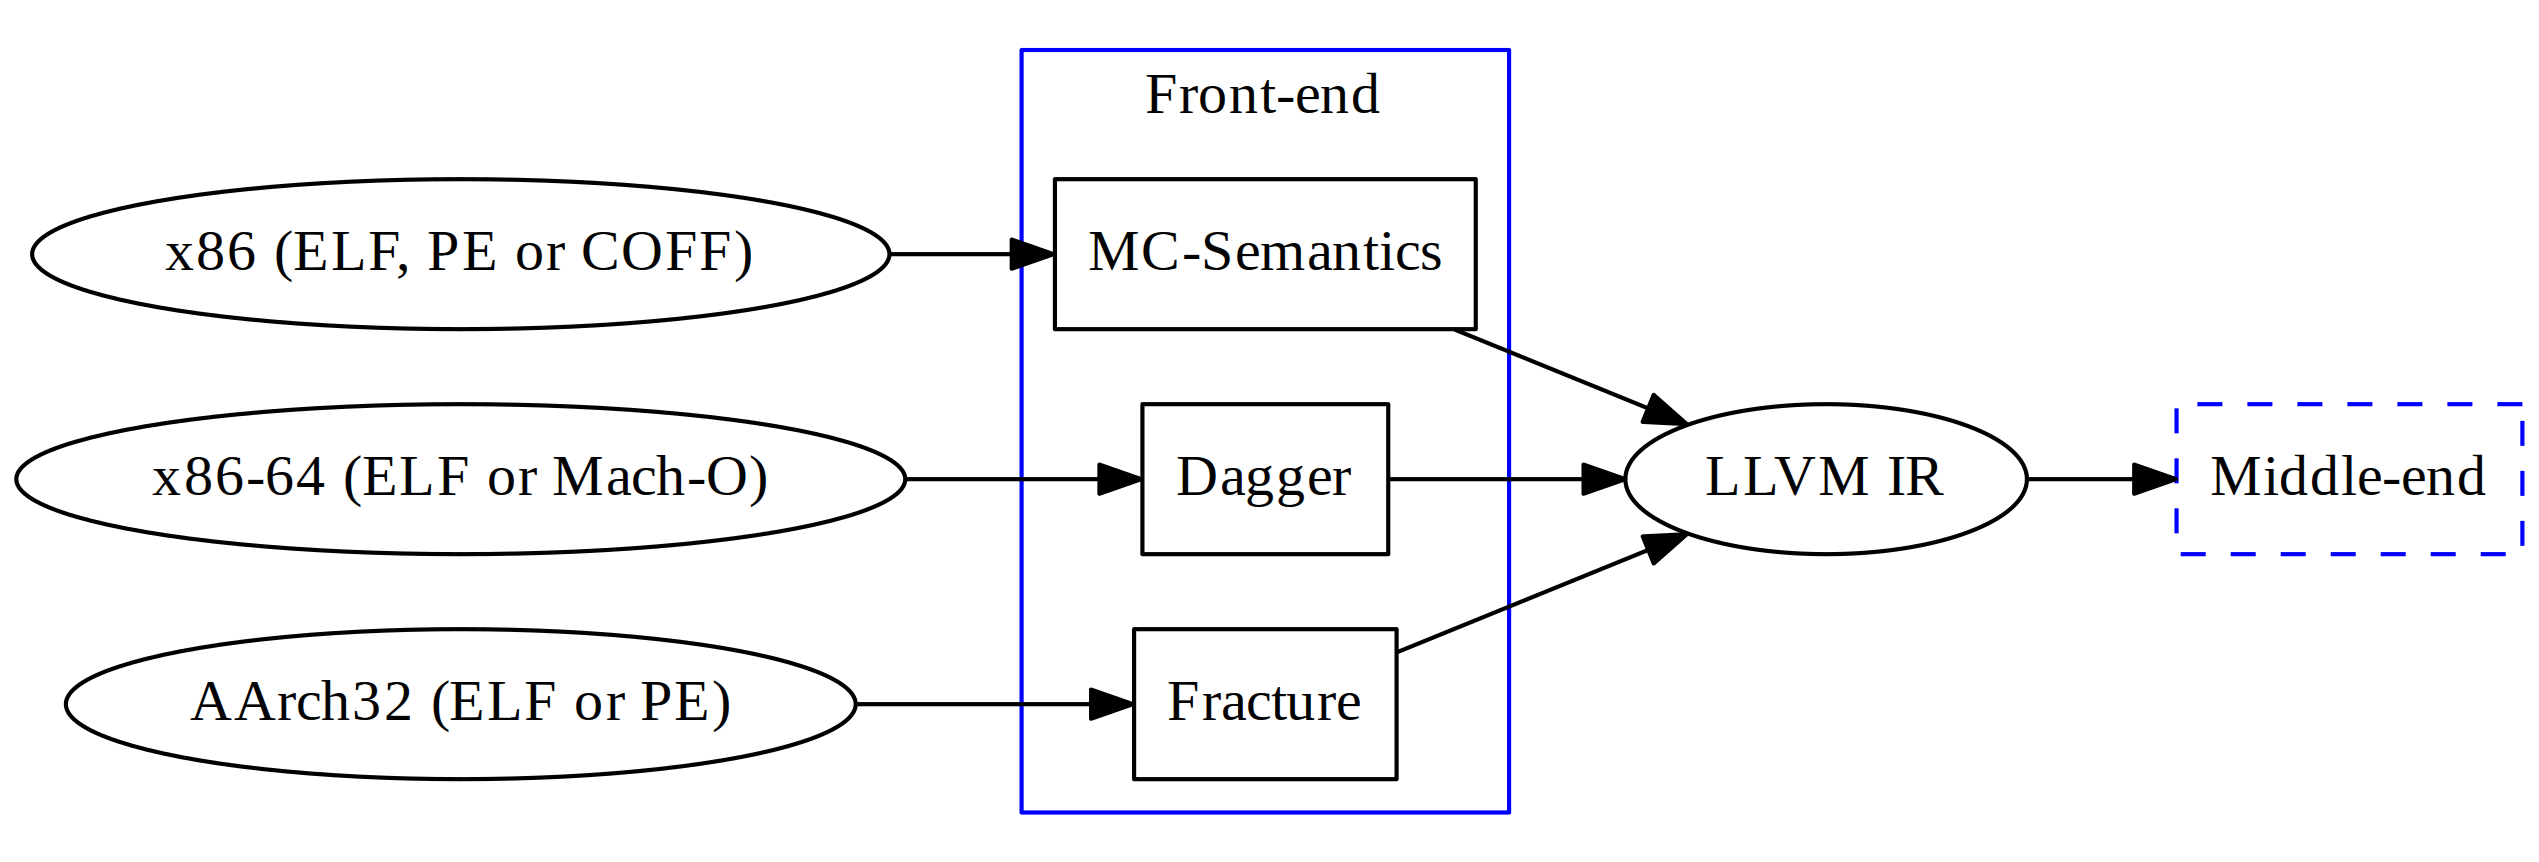
\includegraphics[width=\textwidth]{inc/6_design/front-end_binary.png}
		\caption{The three open source projects MC-Semantics, Dagger and Fracture translate native code of various architectures (e.g. x86, x86-64 and ARM) and file formats (e.g. ELF, PE, COFF and Mach-o) to LLVM IR.}
		\label{fig:front-end_binary}
	\end{center}
\end{figure}
